\section{Enunciado}

\begin{figure}[H]
    \centering
    \fbox{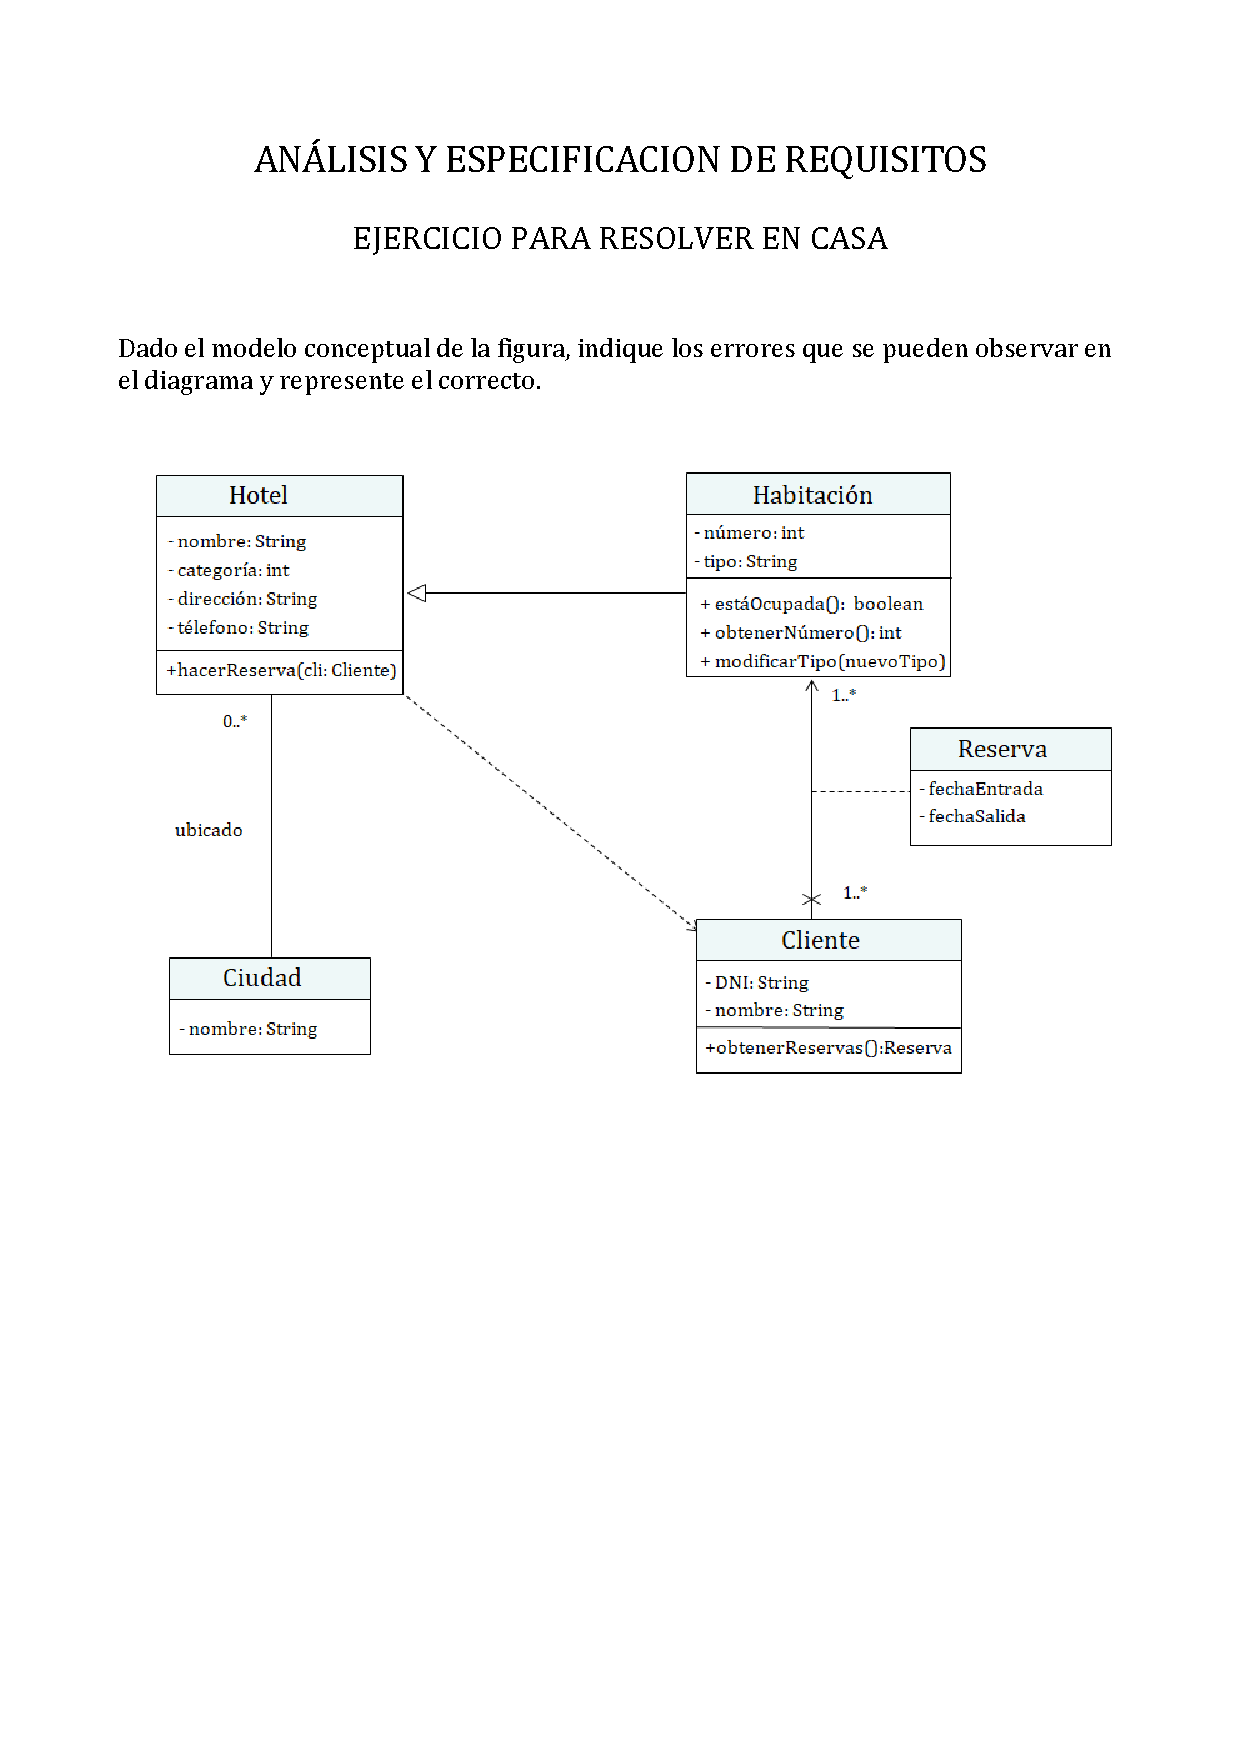
\includegraphics[width=0.8\textwidth,height=0.8\textheight,keepaspectratio]{figures/Ejercicio.pdf}}
    \caption{Enunciado del Ejercicio}
    \label{fig:pdf}
\end{figure}

\newpage
\section{Solución}


Los errores que podemos ver en el modelo conceptual son:
\begin{itemize}
    \item Solo podemos poner atributos, por lo que los métodos deben de eliminarse, de manera análoga pasa con los tipos de los atributos.
    \item Las relaciones son simple, por lo que las flechas no se pueden representar con un triángulo al final, es erróneo en cuanto a la sintaxis (navegabilidad).
    \item La relación de Cliente y Reserva debe de ser 1  a muchos, ya que al tener reserva, una reserva solo puede tener asociado a un cliente.
    % \item La relación de Hotel y Ciudad debe de ser 1 a muchos, ya que una ciudad puede contener muchos hoteles.
    \item Todas las relaciones deben de tener un nombre, como es el caso de la relación entre Hotel y Ciudad.  En mi caso se quedaría de igual manera al usar una relación de composición, ya que en este caso y en el de la la relación de Habitación y Hotel, no es necesario, ya que el significado suele estar implícito en el propio modelado. 
    \item Podemos considerar que un hotel es una composición de habitaciones, por lo tanto, podemos poner una relación de composición en esta.
    \item La relación de dependencia entre Hotel y Cliente es redundante según la teoría, por ello no es necesario ponerla.
\end{itemize}
\newpage

La representación del modelo conceptual quedaría de la siguiente manera:

\begin{figure}[H]
    \centering
    \fbox{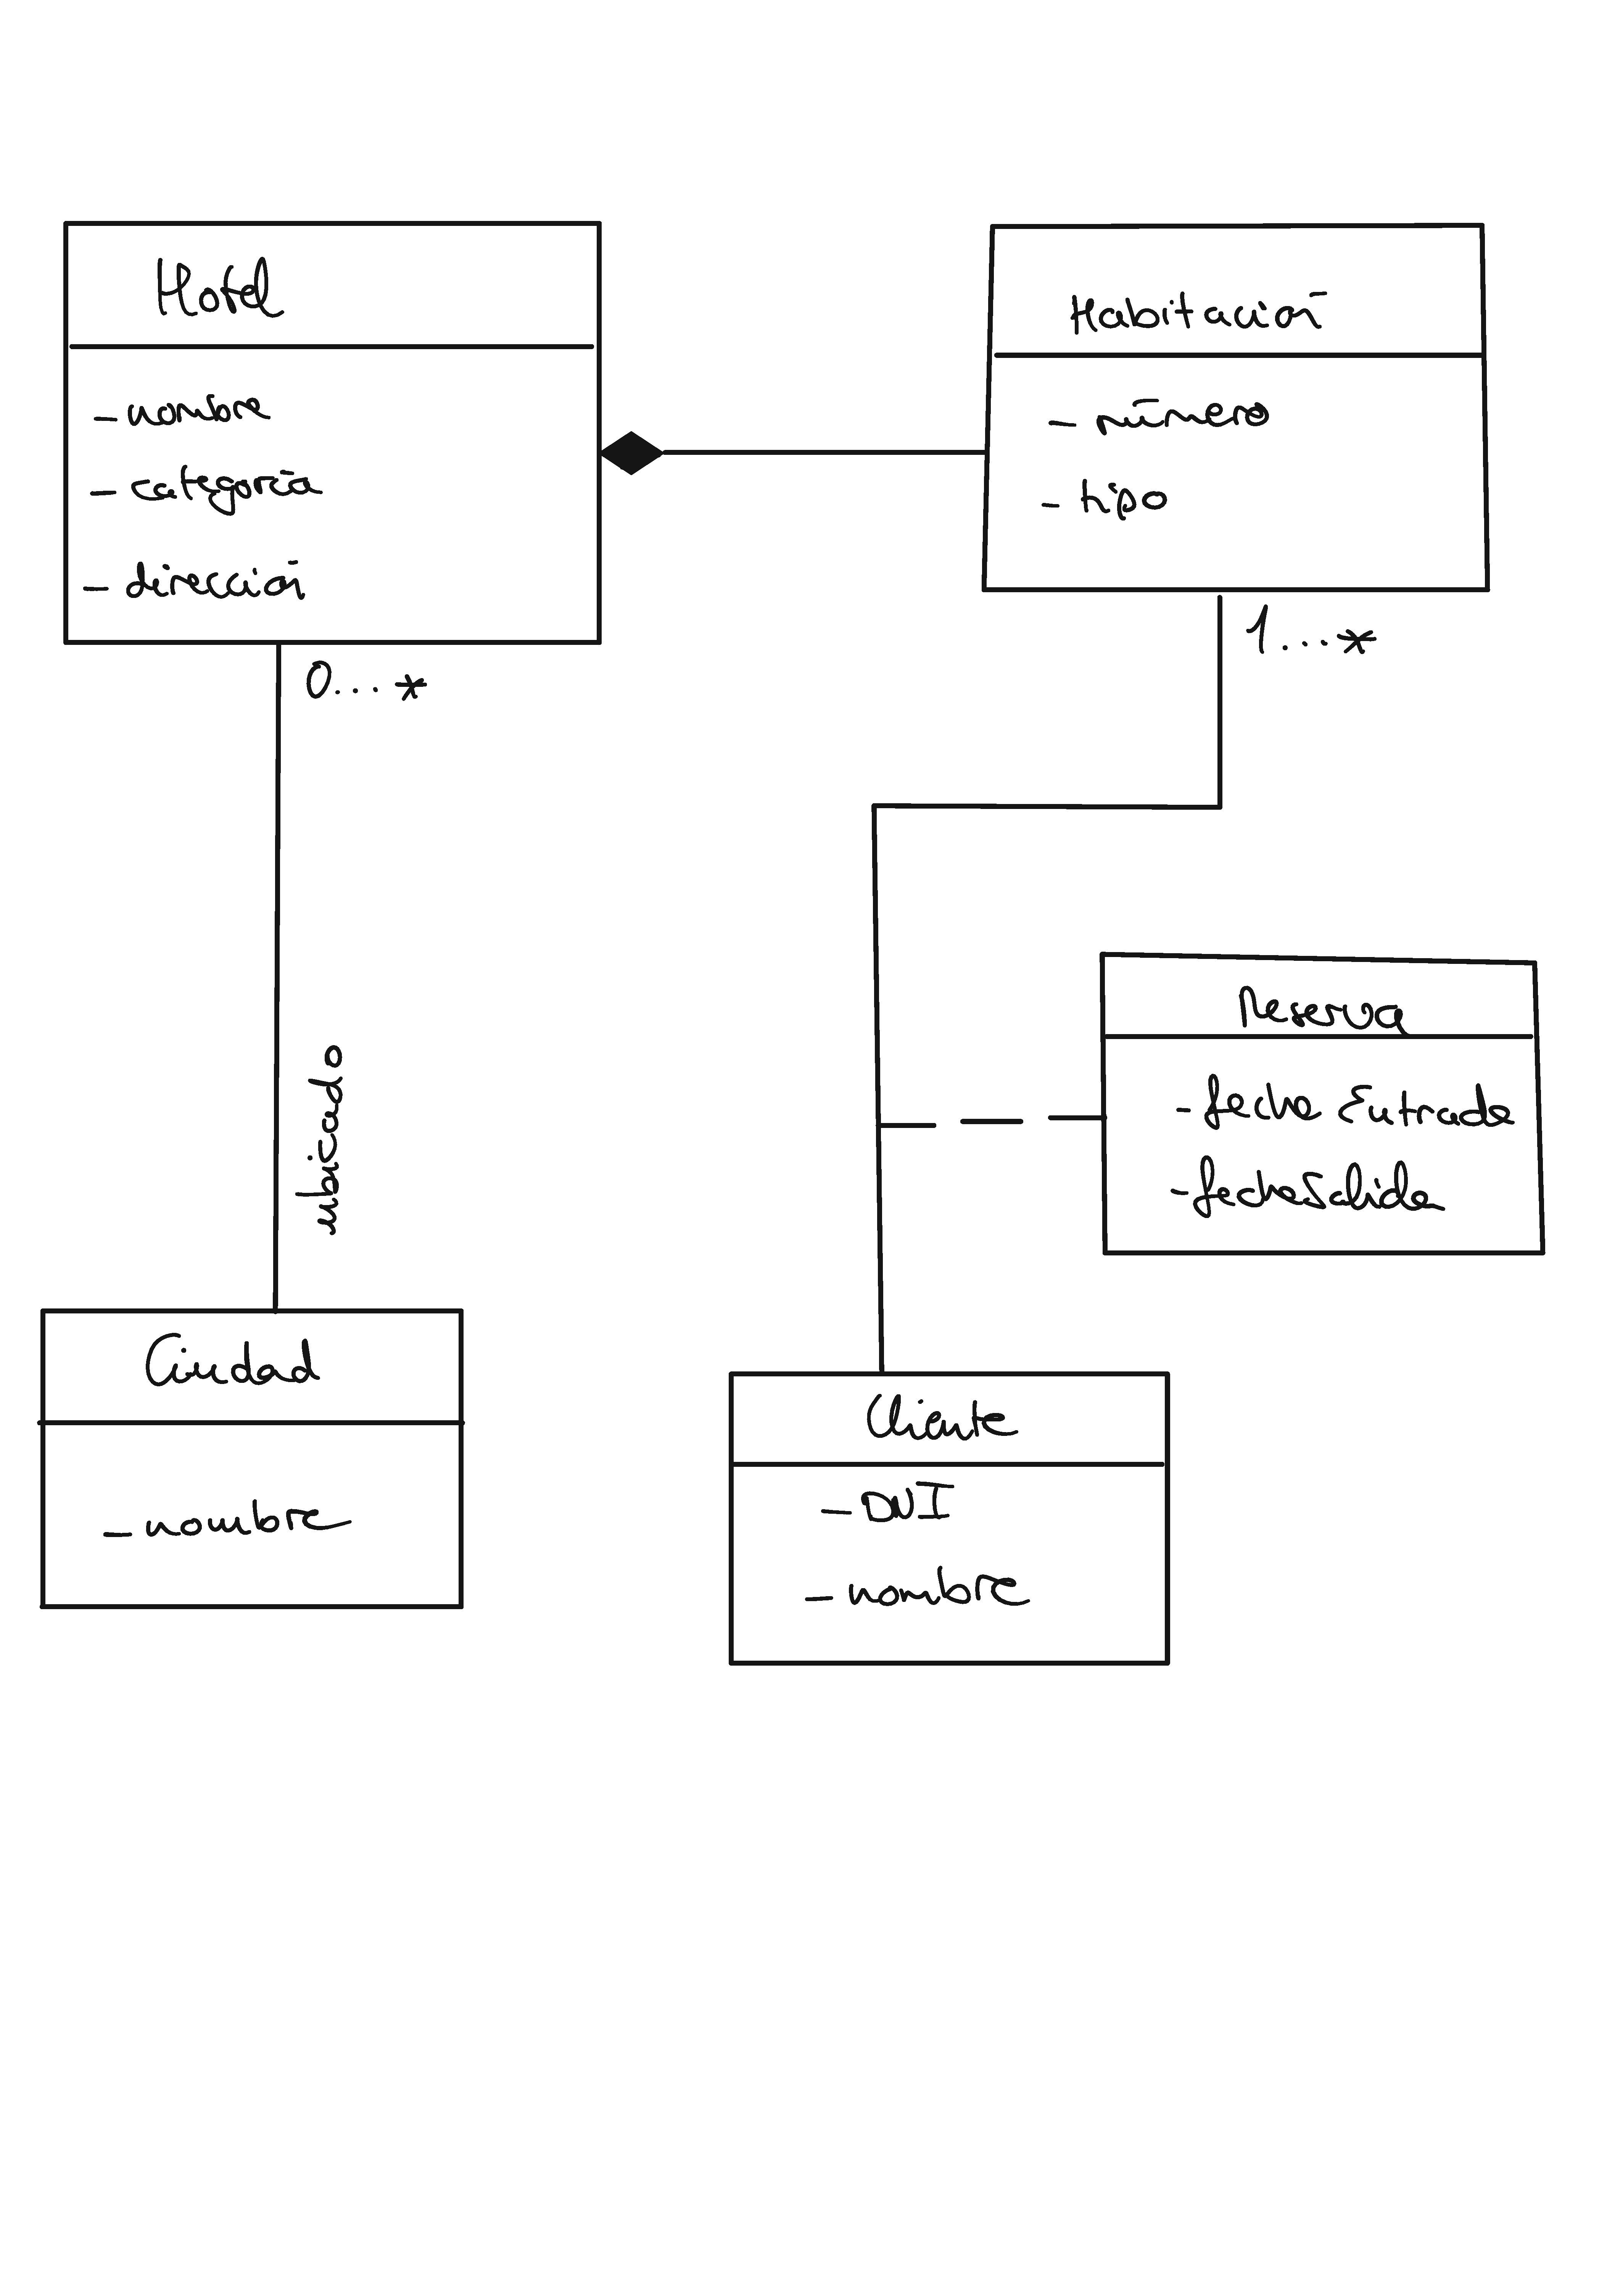
\includegraphics[width=0.8\textwidth,height=0.8\textheight,keepaspectratio]{figures/Solucion.pdf}}
    \caption{Solucion del Ejercicio}
    \label{fig:sol}
\end{figure}